Durch die unterschiedlichen Umlaufzeiten der Planeten um die Sonne wird eine
Umrechnung der Zeit auf der Erde zu der Zeit auf dem Mars ben{\"o}tigt.
Dadurch k{\"o}nnen auf dem Mars aufgenommene Daten eindeutig zugeordnet
werden.
F{\"u}r diese Berechnung wird das heliozentrische Weltbild (die Erde dreht sich
um die Sonne) genutzt, wodurch die Sonne zum gemeinsamen Bezugspunkt f{\"u}r
Erde und Mars wird.

Die Erde bewegt sich mit einer Geschwindigkeit von $27 km/s$ auf einer
elliptischen aber fast kreisf{\"o}rmigen Umlaufbahn um die Sonne (siehe Bild
\ref{fig:marsEarthOrbit}).

\begin{figure}[H]
	\centering
	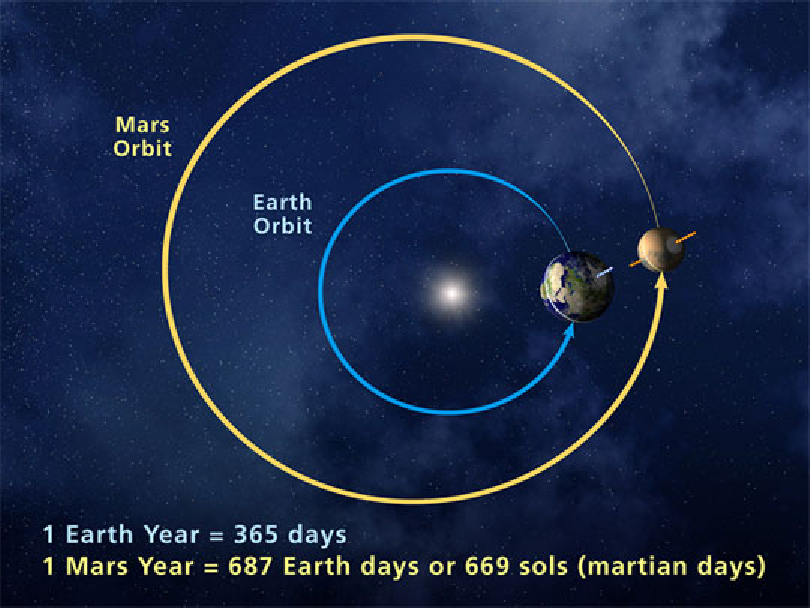
\includegraphics[scale=.5]{earthmarsorbittop.pdf}
	\label{fig:marsEarthOrbit}
	\caption[Umlaufbahn von Erde und Mars]{Umlaufbahn von Erde und Mars \cite{img1}}
\end{figure}

Die Drehrichtung ist rechtl{\"a}ufig. Das hei{\ss}t die Bewegung erfolgt
entgegen dem Uhrzeigersinn um die Sonne. Mit gleichem Drehsinn erfolgt eine Eigenrotation
der Erde. Diese wird als sidierischer Tag bezeichnet und ist nach $23$ Stunden
und $56$ Minuten vollzogen. Die fehlenden $4$ Minuten zu dem uns gel{\"a}ufigen
$24$ Stunden-Tag (Sonnentag) lassen sich durch {\"a}u{\ss}ere Einwirkungen,
wie die Anziehungskraft der Sonne, erkl{\"a}ren. Von dieser Betrachtung
ausgehend, ben{\"o}tigt die Erde f{\"u}r einen einmaligen Umlauf um die Sonne
$365.2424$ Sonnentage, was einem Erdenjahr (tropisches Jahr) oder einem
terrianischen Jahr entspricht.

Die selben Voraussetzungen gelten f{\"u}r den Mars. Die Abbildung
\ref{fig:marsEarthOrbit} zeigt f{\"u}r den Mars eine elliptischere Bahn
auf. Dies hat eine Verschiebung der Tages- und Jahreszeiten zur Folge. Somit ist
auf dem Mars ein Sonnentag exakt $24$ Stunden, $39$ Minuten und $35.24$ Sekunden lang und
wird "`Sol"' (Sol, engl. solar day) genannt. Nach $686.9710$ Erd-Sonnentagen
bzw. $669$ Sol hat der Mars die Sonne einmal vollst{\"a}ndig umkreist. Um eine Beziehung
und somit eine Umrechnung der Zeiten zwischen Planeten vorzunehmen, muss die
Einteilung der Monate und Jahreszeiten aus Sicht der Sonne vorgenommen werden.

Im Weiteren wird eine M{\"o}glichkeit zur Umrechnung der Erdzeit auf Marszeit
nach Robert Zubrin, vorgestellt welcher auch den Begriff "`Sol"'
f{\"u}r einen Marstag pr{\"a}gte. Die nachfolgende Abbildung zeigt den von Zubrin entwickelten
Marskalender (Abbildung \ref{fig:marsEarthCalendar} links) im Vergleich zu dem
bekannten gregorianischen Kalender. Die Monate sind hierbei zur einheitlichen
Bestimmung in Form der lat. Namen der Tierkreiszeichen benannt, welche zu jener
Zeit von der Sonne aus gesehen durchzogen werden.

\begin{figure}[H]
	\centering
	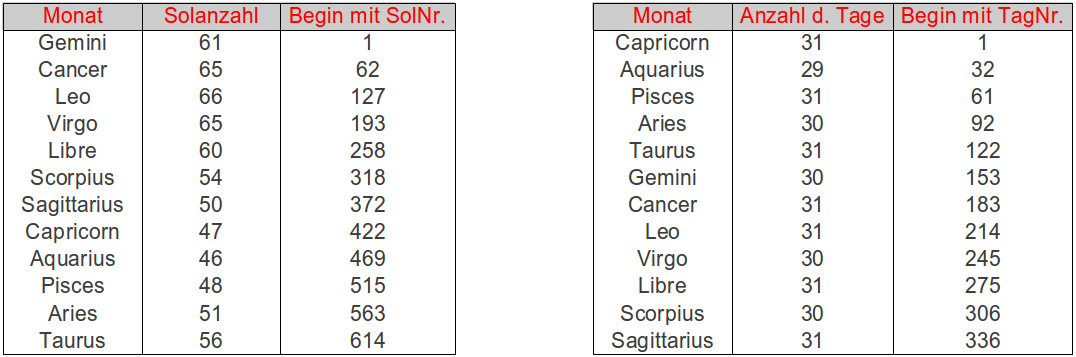
\includegraphics[width=\textwidth]{marsEarthCalendar.png}
	\label{fig:marsEarthCalendar}
	\caption[Kalender: Mars und Erde]{Kalender: Mars und Erde \cite{img2}}
\end{figure}

Bei der Umrechnung zwischen diesen beiden Kalendern bezog sich Zubrin auf das
Jahr $1965$. Dort fielen der Beginn des Erdenjahres ($1.$ Januar), sowie der
Beginn des Marsjahres ($1.$ Gemini) aufeinander. Daraus ergab sich der
nachfolgende Ansatz:

\begin{equation}
	Marsjahr \quad = \quad \left(\frac{8}{15}\right) \quad * \quad (Erdenjahr -
	1961) \quad + \quad 1
	\label{eq:marsYear}
\end{equation}

Das Erdenjahr folgt einer dezimalen Darstellung und setzt sich wie in Formel
\ref{eq:earthYear} zusammen. Zum Tragen kommen hierbei das aktuelle Jahr sowie
die numerischen Angaben von Tag ($numAktTag$) und Monat ($numAktMonat$) des
umzurechnenden Datums. Dies wird ins Verh{\"a}ltnis zur Gesamtanzahl der Tage in
einem Jahr gesetzt.

\begin{equation}
	Erdenjahr \quad = \quad aktuelleJahr + \frac{ (numAktMonat - 1) * 30.4 +
	(numAktTag - 1) }{365}
	\label{eq:earthYear}
\end{equation}

Diese soll am Beispiel der Marslandung des Rovers \textit{Curiosity} am
$6.$ August $2012$ verdeutlicht werden.

Aus Gleichung \ref{eq:earthYear} wird zun{\"a}chst das dezimale Erdenjahr
berechnet.
Es ergibt sich:

\begin{eqnarray}
	Erdenjahr \quad & = & \quad 2012 + \frac{ (8-1) * 30.4 + (6-1) }{365} \\
	Erdenjahr \quad & = & \quad 2012 + 0.59 \\
	Erdenjahr \quad & = & \quad 2012.59
\end{eqnarray}

und in die Gleichung \ref{eq:marsYear} eingesetzt

\begin{eqnarray}
	Marsjahr \quad & = & \quad \left(\frac{8}{15}\right) * (2012.59 - 1961) + 1 \\
	Marsjahr \quad & = & \quad 28.51
\end{eqnarray}

folgt das Marsjahr $28$. Der jeweilige Tag und Monat des Jahres wird
schlussendlich durch die Gleichung \ref{eq:MarsMonthSol} und die Tabelle
\ref{fig:marsEarthCalendar} bestimmt.

\begin{eqnarray}
	Marstag \quad & = & \quad \#MarstageImJahr * restMarsjahr \\
	Marstag \quad & = & \quad 666 * 0.51 \\
	Marstag \quad & = & \quad 340 Sol 
	\label{eq:MarsMonthSol}
\end{eqnarray}

Damit ist die Marssonde \textit{Curiosity} am $22.$ Sol im Sternbild Scorpius
des Marsjahres $28$ auf dem Mars gelandet.

Zubrin's Ansatz weist einige Fehler auf, die auf den ersten Blick keine
gr{\"o}{\ss}eren Probleme verursachen, aber auf weite Sicht starke
Verschiebungen der Zeiten zur Folge haben. Die Annahme, ein Erdenjahr sei immer $365$ Tage lang (siehe Formel
\ref{eq:earthYear}), kann nicht verallgemeinert werden. Vielmehr muss von einem
Mittel ausgegangen werden, da die L{\"a}nge eines Erdenjahres aufgrund der sich
wechselnden Abst{\"a}nde zur Sonne variiert. Hier wird das sogenannte Tropische Jahr
herangezogen, welches $365.2424$ Tage lang ist. Davon ausgehend ist eine
Korrektur des in der Formel \ref{eq:earthYear} angenommenen Verh{\"a}ltnisses von
Mars- zu Erdenjahr (erster Term) auf $\frac{7.97}{15}$ notwendig (Nachweis ab
Formel \ref{eq:errorKorrektur}).

\begin{eqnarray}
	\frac{MarsJahr}{ErdenJahr} \quad & = & \quad \frac{686.9710 \ Tage}{365.2424 \
	Tage}
	\\
	\label{eq:errorKorrektur}  
	\frac{MarsJahr}{ErdenJahr} \quad & = & \quad 1.88 \\
	\notag\\
	x \quad & = & \quad \frac{15}{1.88} \\
	x \quad & = & \quad 7.97 
\end{eqnarray}

Damit w{\"u}rde sich das Landungsdatum der Marssonde auf den $16.$ Sol im Sternbild
Libre verschieben. Nach nur knapp $50$ Jahren der Zeitrechnung Mars stellt sich
bereits eine Verschiebung von $66$ Sol (\ca 1 Marsmonat) ein. Dies zeigt, dass
eine exakte Umrechnung der Daten notwendig ist, um eine langfristige und exakte
Angabe {\"u}ber das Datum und die Zeit auf dem Mars machen zu k{\"o}nnen
\cite{web10}.
